

Décrire votre travail (environ 6 pages)
\begin{itemize}
	\item architecture de votre solution (vision haut niveau)
	\item implémentation de votre solution (détail technique) ou de la partie la plus intéressante si la place manque

\end{itemize}
\newpage
\section{Softwares installation}
In this part I will discuss the different softwares I have installed for the company.
As I said in the previous part, the company needed a tool for project managing and asked
me to install Redmine's software. 
Firstofall I will focus on the researches I have done and the plugins I finally
installed. 
Then the details of the installation will be presented. To finish I will explain how I set
up the environment and how team members can now work with this new software. 
\subsection{Researches}

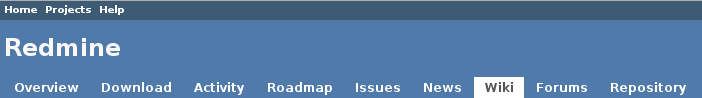
\includegraphics[width=\textwidth, height=70px]{Images/redmine.png}
\newline
\\
I dind't know a lot about project managing so I had to look what was Redmine for and what
 this application will allow the developers to do.  
Redmine is a powerful web based project managing which allow bugs tracking. It allows the
users to create a collection of issues and then see a Gant chart given by the start and 
end dates of issues. You can also look at a calendar to see what happened on a particular
day. The best thing about Redmine is that it is very easy to use. When working on a issue
for example you can update it in one click or add notes to it very quickly. 
 It is possible to add a lot of functionalities to this application by intalling some 
 plugings into it. 

This open-source software is written in Ruby and to install it we need to have the right versions of
Ruby and Rails, depending of the redmine version we want.  

 The developers team needed to keep a track of building versions of their application.
 They also needed to have access to Redmine from Eclipse in order to see and change 
 some issues from their IDE for example. 
I read about all the plugings for Redmine and I finally chose some of them. 
Here is a quick presentation of these plugins :  

	 

\newpage


		
\includegraphics[scale=0.1]{Images/jenkins.jpeg} 
		Jenkins.

		This plugin was quite easy to choose, it fills exactly the need of the 
		company. 
		This application provides an easy to use continuous integration system. 
		It is an application that monitors executions of repeated jobs such as bulding, testing a software project.
		It has 3 main features : 
		\begin{itemize}
			\item It allows a team to share common information easily.
			\item It executes automatically compilation, testing without human intervention.
			\item It keeps a track of previous productions and allow us to see their development. 
		\end{itemize}


		
\includegraphics[scale=0.2]{Images/mylin.jpeg} 
		Mylin for eclipse connection. 

		Here too, the plugin fits exactly the need of the company. It is the only
		one that allow users to have a connection to Redmine from Eclipse.
		Mylin is the task and application lifecycle management framework for Eclipse.
		It allows to visualize tasks from Redmine repository and it has a 
		connector to Jenkins. \\ 
		It helps a developer to work efficiently with many different tasks 
		(such as bugs, problem reports or new features). In a nutshell, 
		it improves their productivity by reducing searching, scrolling, and 
		navigation. \\

		
\includegraphics[scale=0.1]{Images/ldap.jpeg} 
		Ldap authentification. 

		Ldap is a protocol that allow us to access and maintain directory services. So we can access to some informations about the users of a network over TCP/IP protocol. 
		With the ldap authentification into redmine, the users don't need to create a Redmine's account but they can directly access into their redmine's project by using their ldap password and login.   
		It just makes the register part into Redmine easier and faster.


\subsection{Implementation}


I installed Redmine in ssh on an other machine. The installation was not very hard but allow me to know better the IT infrastructure. 
To have an access to Redmine we neeed to run a server. But it's a bit annoying to have to start the server every day or even more. 
That's why I searched how we can start a server automatically when we power up the computer. 
I add a daemon for the Redmine's server, and we can access to our Redmine instance directly. \\ 

Then I installed Jenkins plugin, meanwhile I learnt about SVN in order to add jobs into Redmine. 
SVN is a software versioning and revision control system, it allows Developers to maintain current and historical versions of files such as source code, web pages, and documentation. \\
 
The hardest part was to integrate Mylin into Eclipse. I needed a while to make it work but finally I just used the generic web connector of Eclipse. 

The integration of ldap authentification into Redmine was straightforward. I just needed to configure the authentification mode with ldap data. \\ 

In a nutshell : Schema

\subsection{Project creation}

The last step was to create an instance for the project and look how to set up the environment in order to be nicest to use. 

I wrote some wiki pages related to the project. I add a jenkins page into the project in order to have an access to Jenkins directly from their project.  
Finally I looked how to create new issues in order to be ready to report bugs into Redmine. 



\cleardoublepage


